\chapter{Einleitung}
Diese Arbeit wird sich mit Zeichnungen von einfachen planaren Graphen in der Ebene beschäftigen. Planare Graphen haben durch die Existenz kreuzungsfreier Einbettungen in gewissem Sinne besonders schöne Zeichnungen. Und so ist eine der Fragen, mit der sich schon viele Mathematiker*innen auseinander gesetzt haben und der auch hier nachgegangen wird: \glqq\textit{How to draw a Graph?}\grqq\cite{tutte63}

Beginnen wir mit Varianten von Einbettungen, die wenige Einschränkungen haben. Bei einer topologischen Zeichnung eines planaren Graphen werden die Kanten als Kurven dargestellt. Hierbei dürfen sich die Kanten nur in den Knoten treffen. Erste Resultate zeigten, dass man diese Kurven auch als Geraden zeichnen kann. So wurde in den Fünfzigern wurde unter anderem von István Fáry gezeigt, dass für jeden planaren Graphen und für jede Wahl eines äusseren Gebietes eine geradlinige und kreuzungsfreie Einbettung existiert \cite{fary48}.

In den Siebzigern betrachtete William Thomas Tutte unter anderem in \cite{tutte63} die Unterklasse der 3-zusam\-men\-hängenden planaren Graphen und zeigte, dass für diese nicht nur geradlinige, sondern \textit{konvexe} Zeichnungen existieren. Bei einer konvexen Einbettung entsprechen die Kantenfogen, die ein Gebiet einschließen, den Randkurven von konvexen Polygonen.

\begin{figure}[h]
	\centering
  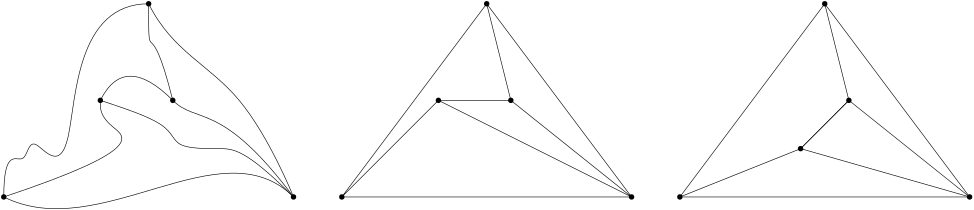
\includegraphics[width=1\textwidth]{topo_straight_convex.png}
	\caption{Der gleiche planare Graph mit einer topologischen, einer geradlinigen einer konvexen und einer geradlinigen Dreiecks Zeichnung.}
	\label{topo_straight_convex}
\end{figure}

Wir werden uns mit einer spezifischen Form dieser Zeichnungen nach Nieke Aerts und Stefan Felsner auseinandersetzten. Es wird gefordert, dass es sich bei eingeschlossenen Polygonen um Dreiecke handelt und das äussere Gebiet ebenfalls dreieckig ist. Wir nennen so eine Darstellung eine \textit{geradlinige Dreiecks Darstellung}. Es ist leicht zu sehen, dass nicht alle planaren Graphen solche Zeichnungen zulassen. Man kann die Klasse der Graphen die eine geradlinige Dreiecks Darstellung zulassen jedoch eingrenzen und Aerts und Felsner haben dies in einigen Publikationen getan \cite{af13h,af13,af15}. Diese Arbeit wir einen Einblick in ihre Resultate liefern.\\

Zum Abschluss der Einleitung folgt ein kurzer Überblick über die Struktur der Arbeit. In Kapitel \ref{pre} werden zunächst einige zur Verständnis der Arbeit wichtige Resultate aus der Graphentheorie wiederholt, die jedoch nicht ein die Grundlagen der Graphentheorie komplett abdecken können. Kapitel \ref{main_theory} befasst sich mit notwendigen und hinreichenden Bedingungen an die Existenz von geradlinigen Dreiecks Darstellungen. In Kapitel \ref{main_algo} wird dann aufbauend auf diesen Ergebnissen ein Algorithmus kreiert um eine geradlinige Dreiecks Darstellung eines planaren Graphen zu berchnen, soweit diese existiert. Abschließend wird in Kapitel \ref{the_program} einen Überblick über Ergebnisse einer Implementierung der erarbeiteten Algorithmen gegeben.